\documentclass[10pt,aspectratio=169]{beamer}

\usetheme[progressbar=frametitle]{metropolis}

\newcommand{\R}{\mathbb{R}}
\renewcommand{\P}{\mathbb{P}}
\newcommand{\set}[1]{\{#1\}}

\usepackage{tikz}
\usetikzlibrary{shapes}
\usetikzlibrary{plotmarks}
\usetikzlibrary{fit}
\usetikzlibrary{overlay-beamer-styles}
\usetikzlibrary{positioning}
\usetikzlibrary{calc}
\usetikzlibrary{decorations.pathreplacing}
\usetikzlibrary{decorations.pathmorphing}
\definecolor{lightblue}{RGB}{189,216,238}

\usepackage{etoolbox}

\title{Non-Parametric Machine Learning Models for Solar Energy Forecasting}
% \subtitle{}
\date{16.07.2021}
\author{Pavel Zwerschke}
\institute{Karlsruhe Institute of Technology}
% \titlegraphic{\hfill\includegraphics[height=1.5cm]{logo.pdf}}

\begin{document}

\maketitle

\begin{frame}{Table of contents}
    \setbeamertemplate{section in toc}[sections numbered]
    \tableofcontents%[hideallsubsections]
\end{frame}

\begin{frame}{Introduction}
    \begin{itemize}
        \item Solar energy generation is characterized by fluctuations due to uncertainty of the weather
        \item Uncertainty should be quantified through a probabilistic forecast
        \begin{itemize}
            \item Probabilistic forecasts for solar energy generation are underdeveloped
            \item[\(\leadsto\)] We want to compare different machine learning based forecasting models on solar power
        \end{itemize}
    \end{itemize}
\end{frame}

\section{Model descriptions}

\begin{frame}{NNQF}
    \begin{center}
        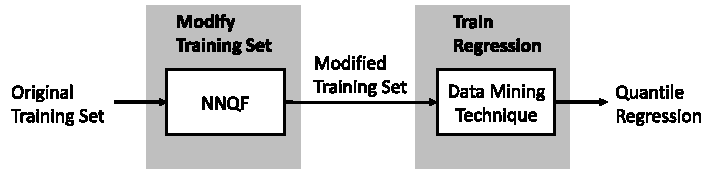
\includegraphics{plots/nnqf_approach.pdf}
    \end{center}
    \begin{itemize}
        \item Let \(x_1, \ldots, x_n \in \R^D\) be the predictors and \(y_1, \ldots, y_n\in \R\) the target values.
        \item Calculate approximate quantiles of \(y_i\):
        \begin{itemize}
            \item Find \(N\) nearest neighbors of \(x_i\): \(\set{y_{i_1}, \ldots, y_{i_N}}\)
            \item Calculate the empirical quantiles \(y_{(0.01)}, \ldots, y_{(0.99)}\) from \(\set{y_{i_1}, \ldots, y_{i_N}}\)
        \end{itemize}
    \end{itemize}
\end{frame}

\begin{frame}{NNQF}
    \begin{itemize}
        \item After modification of training set, a data mining technique is used for learning the map \(f(x) = (y_{(0.01)}, \ldots, y_{(0.99)})\).
        \item High correlation of adjacent data points \(\leadsto\) don't just use \(x_i\) for prediction of \(y_i\), but also 
        \(x_{i-1}, \ldots, x_{i-H+1}\)
    \end{itemize}
\end{frame}

\begin{frame}{Advantages of NNQF}
    \begin{itemize}
        \item \(q\) is a free parameter and can be changed to any \(q\in (0,1)\)
        \item the regression technique is not specified, any technique can be used
        \item nearest neighbor calculation only needs to be done once
        \item the original dataset does not need to be saved
    \end{itemize}
\end{frame}

\begin{frame}{QRF}
    \begin{itemize}
        \item Use bagging to produce \(k\) trees from training set \(x_1, \ldots, x_n \in \R^D\) and \(y_1, \ldots, y_n \in \R\)
        \item For \(x\in \R^D\), we want to predict the distribution \(\P(Y | X=x)\)
        \begin{itemize}
            \item Calculate \(\hat{y}_1, \ldots, \hat{y}_k\) from the trees 
            \item Calculate the empirical quantiles \(\hat{y}_{(q)}\) of \(\set{\hat{y}_1, \ldots, \hat{y}_k}\) for any \(q \in (0,1)\)
        \end{itemize}
        \item[\(\leadsto\)] Basically like Random Forests but instead of calculating the mean, you calculate the quantiles of the prediction
    \end{itemize}
\end{frame}

\begin{frame}{DeepAR -- Training}
    \centering
    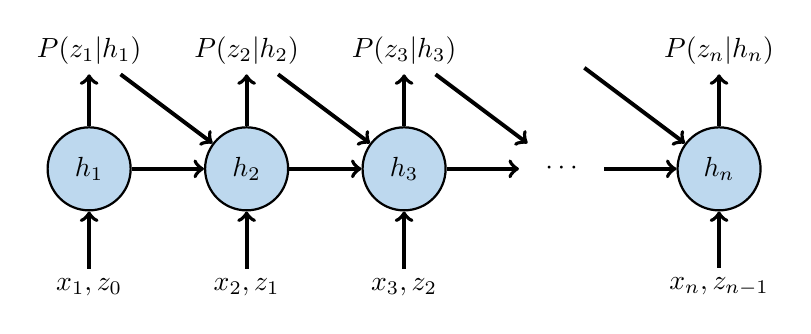
\begin{tikzpicture}
        \node[circle, draw=black, fill=lightblue, thick, inner sep=2pt, minimum size=30pt] (circ1) at (0, 0) {\(h_1\)};
        \node (x1) at (0, -1.5) {\(x_1, z_0\)};
        \draw[->, line width=0.5mm] (x1) -- (circ1);
        \node (y1) at (0, 1.5) {\(\P(z_1|h_1)\)};
        \draw[->, line width=0.5mm] (circ1) -- (y1);

        \node[circle, draw=black, fill=lightblue, thick, inner sep=2pt, minimum size=30pt] (circ2) at (2, 0) {\(h_2\)};
        \node (x2) at (2, -1.5) {\(x_2, z_1\)};
        \draw[->, line width=0.5mm] (x2) -- (circ2);
        \node (y2) at (2, 1.5) {\(\P(z_2|h_2)\)};
        \draw[->, line width=0.5mm] (circ2) -- (y2);

        \node[circle, draw=black, fill=lightblue, thick, inner sep=2pt, minimum size=30pt] (circ3) at (4, 0) {\(h_3\)};
        \node (x3) at (4, -1.5) {\(x_3, z_2\)};
        \draw[->, line width=0.5mm] (x3) -- (circ3);
        \node (y3) at (4, 1.5) {\(\P(z_3|h_3)\)};
        \draw[->, line width=0.5mm] (circ3) -- (y3);

        \node[circle, opacity=0, thick, inner sep=2pt, minimum size=30pt] (circ4) at (6, 0) {};
        \node at (circ4) {\(\cdots\)};
        \node[opacity=0] (y4) at (6, 1.5) {\(y_4\)};

        \node[circle, draw=black, fill=lightblue, thick, inner sep=2pt, minimum size=30pt] (circn) at (8, 0) {\(h_n\)};
        \node (xn) at (8, -1.5) {\(x_n, z_{n-1}\)};
        \draw[->, line width=0.5mm] (xn) -- (circn);
        \node (yn) at (8, 1.5) {\(\P(z_n|h_n)\)};
        \draw[->, line width=0.5mm] (circn) -- (yn);

        \draw[->, line width=0.5mm] (circ1) -- (circ2);
        \draw[->, line width=0.5mm] (y1) -- (circ2);
        \draw[->, line width=0.5mm] (circ2) -- (circ3);
        \draw[->, line width=0.5mm] (y2) -- (circ3);
        
        \draw[->, line width=0.5mm] (circ3) -- (circ4);
        \draw[->, line width=0.5mm] (y3) -- (circ4);
        \draw[->, line width=0.5mm] (circ4) -- (circn);
        \draw[->, line width=0.5mm] (y4) -- (circn);
    \end{tikzpicture}
\end{frame}

\begin{frame}{DeepAR -- Predicting}
    \centering
    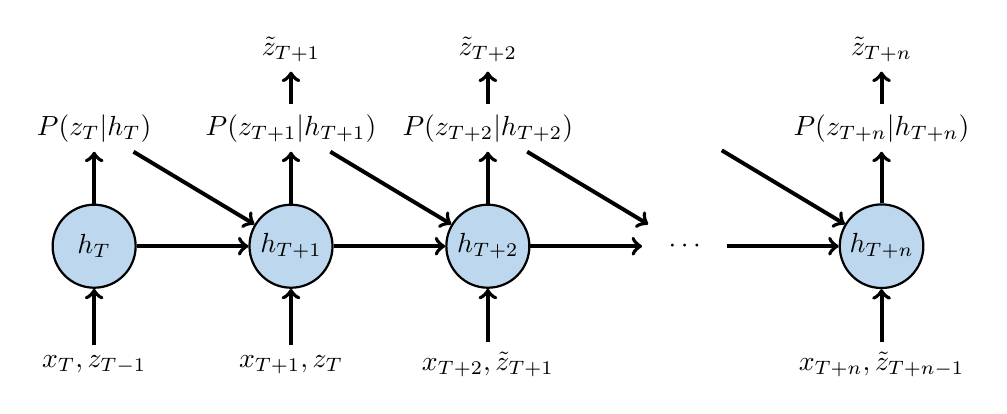
\begin{tikzpicture}
        \node[circle, draw=black, fill=lightblue, thick, inner sep=2pt, minimum size=30pt] (circ1) at (0, 0) {\(h_T\)};
        \node (x1) at (0, -1.5) {\(x_T, z_{T-1}\)};
        \draw[->, line width=0.5mm] (x1) -- (circ1);
        \node (y1) at (0, 1.5) {\(\P(z_T|h_T)\)};
        \draw[->, line width=0.5mm] (circ1) -- (y1);

        \node[circle, draw=black, fill=lightblue, thick, inner sep=2pt, minimum size=30pt] (circ2) at (2.5, 0) {\(h_{T+1}\)};
        \node (x2) at (2.5, -1.5) {\(x_{T+1}, z_T\)};
        \draw[->, line width=0.5mm] (x2) -- (circ2);
        \node (y2) at (2.5, 1.5) {\(\P(z_{T+1}|h_{T+1})\)};
        \draw[->, line width=0.5mm] (circ2) -- (y2);
        \node (z2) at (2.5, 2.5) {\(\tilde{z}_{T+1}\)};
        \draw[->, line width=0.5mm] (y2) -- (z2);

        \node[circle, draw=black, fill=lightblue, thick, inner sep=2pt, minimum size=30pt] (circ3) at (5, 0) {\(h_{T+2}\)};
        \node (x3) at (5, -1.5) {\(x_{T+2}, \tilde{z}_{T+1}\)};
        \draw[->, line width=0.5mm] (x3) -- (circ3);
        \node (y3) at (5, 1.5) {\(\P(z_{T+2}|h_{T+2})\)};
        \draw[->, line width=0.5mm] (circ3) -- (y3);
        \node (z3) at (5, 2.5) {\(\tilde{z}_{T+2}\)};
        \draw[->, line width=0.5mm] (y3) -- (z3);

        \node[circle, opacity=0, thick, inner sep=2pt, minimum size=30pt] (circ4) at (7.5, 0) {};
        \node at (circ4) {\(\cdots\)};
        \node[opacity=0] (y4) at (7.5, 1.5) {\(\tilde{y}_{T+3}\)};

        \node[circle, draw=black, fill=lightblue, thick, inner sep=2pt, minimum size=30pt] (circn) at (10, 0) {\(h_{T+n}\)};
        \node (xn) at (10, -1.5) {\(x_{T+n}, \tilde{z}_{T+n-1}\)};
        \draw[->, line width=0.5mm] (xn) -- (circn);
        \node (yn) at (10, 1.5) {\(\P(z_{T+n}|h_{T+n})\)};
        \draw[->, line width=0.5mm] (circn) -- (yn);
        \node (zn) at (10, 2.5) {\(\tilde{z}_{T+n}\)};
        \draw[->, line width=0.5mm] (yn) -- (zn);

        \draw[->, line width=0.5mm] (circ1) -- (circ2);
        \draw[->, line width=0.5mm] (y1) -- (circ2);
        \draw[->, line width=0.5mm] (circ2) -- (circ3);
        \draw[->, line width=0.5mm] (y2) -- (circ3);
        
        \draw[->, line width=0.5mm] (circ3) -- (circ4);
        \draw[->, line width=0.5mm] (y3) -- (circ4);
        \draw[->, line width=0.5mm] (circ4) -- (circn);
        \draw[->, line width=0.5mm] (y4) -- (circn);
    \end{tikzpicture}
\end{frame}

\begin{frame}{SQF-RNN}
    \begin{center}
        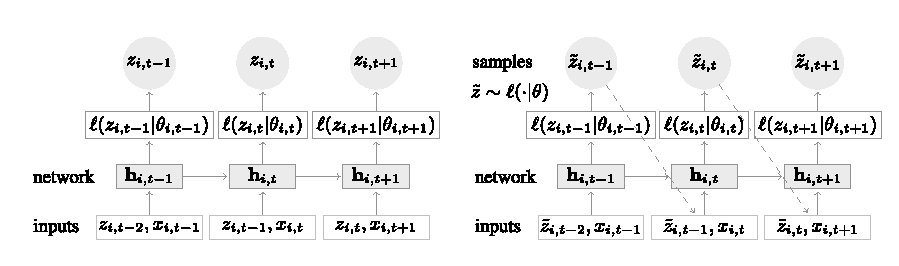
\includegraphics[width=\textwidth]{plots/deepar-rnn.pdf}
    \end{center}
    \begin{itemize}
        \item Autoregressive Recurrent Neural Network with probabilistic output
        \item \(x_{i, t}\) and \(z_{i, t-1}\) form with \(\boldsymbol{h}_{i,t-1}\) the new network output \(\boldsymbol{h}_{i,t}\)
        which is used to compute \(\theta_{i,t}\) and the likelihood \(\ell(z_{i,t} | \theta_{i,t})\)
        \item Generate \(\tilde{z}_{i, t} \sim \ell(\cdot | \theta_{i,t})\) for testing from previous step
    \end{itemize}
\end{frame}

\begin{frame}{SQF-RNN}
    \begin{itemize}
        \item Output distribution is given by monotonously increasing linear splines: 
        \[ s(x; \gamma, b, d) = \gamma + \sum_{l=0}^L b_l (x - d_l)_+ \]
        \item Arbitrary distribution can be fit \(\leadsto\) no assumption on distribution
    \end{itemize}
\end{frame}

\section{Comparison}

\begin{frame}{Pinball loss}
    
\end{frame}

\begin{frame}{Energy score}
    
\end{frame}

\begin{frame}{Feature importance}
    
\end{frame}

\section{Conclusion}

\begin{frame}{Conclusion}
    
\end{frame}

\end{document}